\documentclass[a4paper, journal]{IEEEtran}
\usepackage[margin=0.75in]{geometry}
\IEEEoverridecommandlockouts
\usepackage{cite}
\usepackage{amsmath,amssymb,amsfonts}
\usepackage{algorithmic}
\usepackage{graphicx}
\usepackage{textcomp}
\usepackage{listings}
\usepackage{xcolor}
\usepackage{booktabs}
\usepackage{tikz}
\usetikzlibrary{shapes,positioning,arrows}
\usepackage{times}
\usepackage{newtxmath}

\definecolor{codegreen}{rgb}{0,0.6,0}
\definecolor{codegray}{rgb}{0.5,0.5,0.5}
\definecolor{codepurple}{rgb}{0.58,0,0.82}
\definecolor{backcolour}{rgb}{0.95,0.95,0.92}

\lstset{
  language=Python,
  breaklines=true,
  breakatwhitespace=true,
  basicstyle=\ttfamily\footnotesize,
  keywordstyle=\color{codepurple},
  commentstyle=\color{codegreen},
  stringstyle=\color{red},
  captionpos=b,
  frame=single,
  showstringspaces=false,
  tabsize=4
}

\usepackage{balance}
\begin{document}

\title{LeNet Convolutional Neural Network for MNIST Handwritten Digit Classification}
\author{
    \IEEEauthorblockN{Dinanath Padhya\IEEEauthorrefmark{1}, Krishna Acharya\IEEEauthorrefmark{2}} \\
    \IEEEauthorblockA{\IEEEauthorrefmark{1}THA078BEI010 \quad \IEEEauthorrefmark{2}THA078BEI020\\
        Department of Electronics, Communication and Information Engineering\\
        Thapathali Campus, IOE, Tribhuvan University, Nepal\\
    }}

\maketitle

\begin{abstract}
    This laboratory experiment implements the LeNet-5 convolutional neural network using the PyTorch framework to classify handwritten digits from the MNIST dataset. The model was trained for five epochs and achieved a test accuracy of 98.50\%, with a steady decline in training and validation losses. These results demonstrate the strength of convolutional layers in capturing spatial hierarchies in image data. In contrast, a traditional Artificial Neural Network (ANN) exhibited lower accuracy and struggled with visual pattern generalization, highlighting its limitations for image-based tasks. The experiment validates LeNet-5’s effectiveness in digit recognition and emphasizes the advantages of convolutional architectures in deep learning for image classification.



\end{abstract}

\begin{IEEEkeywords}
    Convolutional Neural Networks, LeNet-5, MNIST, PyTorch, Image Classification, Deep Learning, ANN, Overfitting, Underfitting
\end{IEEEkeywords}

\section{Introduction}

LeNet-5 , introduced by Yann LeCun et al. in 1998, is one of the earliest and most influential convolutional neural network architectures \cite{lecun1998gradient}. Originally designed for handwritten digit recognition, it established the fundamental building blocks that are still used in modern deep learning: convolutional layers, pooling layers, and fully connected layers. The MNIST dataset, consisting of 70,000 grayscale images of handwritten digits (0-9), serves as an ideal testbed for evaluating the performance of this classic architecture.

\subsection{Objectives}

The primary objectives of this laboratory experiment are:
\begin{itemize}
    \item Implement the LeNet-5 architecture using PyTorch framework
    \item Train the model on MNIST handwritten digit dataset
    \item Analyze the effectiveness of convolutional neural networks for image classification
\end{itemize}

\section{Methodology}

\subsection{LeNet-5 Architecture}

LeNet-5 is a feedforward neural network with the following layer structure shown in Table~\ref{tab:lenet_arch}:

\subsubsection{Convolution Output Size Calculation}

The output dimensions after a convolution operation can be calculated using the following formula:

\begin{equation}
    O = \frac{I + 2P - K}{S} + 1
\end{equation}

where:
\begin{itemize}
    \item $O$ = Output size (height or width)
    \item $I$ = Input size (height or width)
    \item $P$ = Padding
    \item $K$ = Kernel size (filter size)
    \item $S$ = Stride
\end{itemize}

For example, in the first convolutional layer of LeNet-5:
\begin{itemize}
    \item Input: 28×28, Kernel: 5×5, Padding: 2, Stride: 1
    \item Output size: $\frac{28 + 2(2) - 5}{1} + 1 = \frac{28 + 4 - 5}{1} + 1 = 28$
    \item Therefore: 28×28×6 output
\end{itemize}

\begin{table}[h]
    \centering
    \caption{LeNet-5 Architecture (Short Form)}
    \label{tab:lenet_arch}    \resizebox{\linewidth}{!}{
        \begin{tabular}{cccc}
            \toprule
            Layer & Type        & Output Size            & Parameters          \\
            \midrule
            Input & -           & 28$\times$28$\times$1  & -                   \\
            Conv1 & Conv + ReLU & 28$\times$28$\times$6  & 5$\times$5, pad=2   \\
            Pool1 & Pool (Avg)  & 14$\times$14$\times$6  & 2$\times$2, s=2     \\
            Conv2 & Conv + ReLU & 10$\times$10$\times$16 & 5$\times$5          \\
            Pool2 & Pool (Avg)  & 5$\times$5$\times$16   & 2$\times$2, s=2     \\
            FC1   & FC + ReLU   & 120                    & 400$\rightarrow$120 \\
            FC2   & FC + ReLU   & 84                     & 120$\rightarrow$84  \\
            FC3   & FC          & 10                     & 84$\rightarrow$10   \\
            \bottomrule
        \end{tabular}
    }
\end{table}

\subsection{Activation Functions}

The network employs ReLU (Rectified Linear Unit) activation functions throughout the hidden layers. ReLU is defined as:
\begin{equation}
    f(x) = \max(0, x)
\end{equation}

ReLU provides several advantages like Computational Efficiency.


\subsection{Loss Functions}

Cross-entropy loss is used for this multi-class classification problem:
\begin{equation}
    \mathcal{L} = -\sum_{i=1}^{N} \sum_{c=1}^{C} y_{i,c} \log(\hat{y}_{i,c})
\end{equation}

where $N$ is the batch size, $C$ is the number of classes (10), $y_{i,c}$ is the true label, and $\hat{y}_{i,c}$ is the predicted probability.

\subsection{Optimizers}

Adam optimizer is employed with a learning rate of 0.001. Adam combines the advantages of AdaGrad and RMSprop:
% \begin{align}
%     m_t          & = \beta_1 m_{t-1} + (1-\beta_1) g_t                               \\
%     v_t          & = \beta_2 v_{t-1} + (1-\beta_2) g_t^2                             \\
%     \hat{m}_t    & = \frac{m_t}{1-\beta_1^t}                                         \\
%     \hat{v}_t    & = \frac{v_t}{1-\beta_2^t}                                         \\
%     \theta_{t+1} & = \theta_t - \frac{\alpha}{\sqrt{\hat{v}_t} + \epsilon} \hat{m}_t
% \end{align}

\subsection{Training and Evaluation Loops}

The training and evaluation process in this experiment adheres to standard deep learning practices. During each epoch, the model performs a forward pass to generate predictions from the input data, followed by the calculation of the loss by comparing these predictions with the true labels using the cross-entropy loss function. The backward pass then computes gradients with respect to the model parameters, and the optimizer \emph{(Adam)} updates the parameters accordingly. After each training epoch, the model is evaluated on the validation set to monitor generalization performance and detect potential overfitting. This iterative process ensures that the model learns effectively from the training data while maintaining robust performance on unseen samples.

\subsection{Dataset}

The MNIST dataset is a widely used benchmark in the field of machine learning and computer vision. It consists of 60,000 training images and 10,000 test images, each representing a handwritten digit from 0 to 9. All images are grayscale and have a fixed resolution of 28×28 pixels, resulting in a compact and standardized input format. The dataset covers 10 distinct classes corresponding to the digits 0 through 9. For effective neural network training, the pixel values are normalized to the range [0,1] using a mean of 0.1307 and a standard deviation of 0.3081, which helps in accelerating convergence and improving model performance.

\subsection{Overfitting, Underfitting, and CNN Advantages Over Traditional ANNs}

\subsubsection{Problems with Traditional ANNs for Image Data}

Traditional Artificial Neural Networks (ANNs), also known as Multi-Layer Perceptrons (MLPs), face significant challenges when applied to image classification tasks, particularly regarding overfitting and the inability to capture spatial relationships inherent in visual data.

\textbf{Overfitting in ANNs:}
When applied to image data, traditional ANNs suffer from severe overfitting due to several fundamental issues:

\begin{itemize}
    \item \textbf{Massive Parameter Count}: For a 28×28 MNIST image, a fully connected network requires 784 input neurons. A modest hidden layer of 256 neurons would require 784×256 = 200,704 parameters just for the first layer. This enormous parameter space leads to memorization rather than generalization.

    \item \textbf{Lack of Spatial Awareness}: ANNs treat each pixel as an independent feature, ignoring the crucial spatial relationships between adjacent pixels that define edges, shapes, and patterns in images.

    \item \textbf{Position Sensitivity}: Traditional ANNs lack translational invariance, meaning a digit shifted by even one pixel would be treated as a completely different input pattern, requiring the network to learn the same features at every possible position.

    \item \textbf{Feature Engineering Burden}: In tabular data, feature engineering is performed manually to create meaningful independent features. However, for images, adjacent pixels are inherently correlated and contain spatial information that ANNs cannot automatically exploit.
\end{itemize}

\subsubsection{How CNNs Address These Limitations}

Convolutional Neural Networks fundamentally solve these problems through specialized architectural components that are specifically designed for visual data processing.

\textbf{Translational Invariance:}
CNNs achieve translational invariance through two key mechanisms:
\begin{itemize}
    \item \textbf{Shared Weights}: Convolutional filters use the same set of weights across all spatial locations, enabling the network to detect the same feature regardless of its position in the image.
    \item \textbf{Pooling Operations}: Pooling layers provide additional translational invariance by summarizing local regions, making the representation robust to small spatial shifts.
\end{itemize}

\textbf{Complexity Reduction and Overfitting Prevention:}
CNNs achieve an optimal balance between model capacity and generalization through:

\begin{enumerate}
    \item \textbf{Parameter Sharing}: A single 5×5 convolutional filter has only 25 learnable parameters but can detect features across the entire image, dramatically reducing the total parameter count compared to fully connected layers.

    \item \textbf{Local Connectivity}: Each neuron connects only to a small local region (receptive field), reducing the number of connections and focusing learning on local patterns.

    \item \textbf{Hierarchical Feature Learning}: Lower layers learn simple features (edges, corners), while deeper layers combine these to form complex patterns (shapes, objects), mimicking the hierarchical processing in biological vision systems.
\end{enumerate}

\subsubsection{Spatial Feature Integration in CNNs}

Unlike tabular data where feature engineering must be performed manually to create meaningful independent features, CNNs automatically handle the spatial correlation inherent in image data:

\textbf{Automatic Feature Engineering:}
\begin{itemize}
    \item \textbf{Convolution Operations}: Systematically scan the image with learned filters to detect local patterns. The mathematical operation is:
          \begin{equation}
              (f * g)(x,y) = \sum_{i=-k}^{k} \sum_{j=-k}^{k} f(i,j) \cdot g(x-i, y-j)
          \end{equation}
          where $f$ is the input image and $g$ is the learned filter.

    \item \textbf{Feature Maps}: Each convolutional layer produces feature maps that highlight specific patterns, creating a rich representation of the input image at different abstraction levels.

    \item \textbf{Spatial Correlation Exploitation}: Adjacent pixels in images are highly correlated and contain spatial information about edges, textures, and shapes. CNNs explicitly model these relationships through local connectivity patterns.
\end{itemize}

\subsubsection{Pooling Operations: Non-Reconstructiveness and Invariance}

Pooling operations serve as crucial components in CNN architectures, providing both dimensionality reduction and important invariance properties:

\textbf{Types and Functions of Pooling:}
\begin{itemize}
    \item \textbf{Average Pooling (used in LeNet)}: Computes the mean value over a local region:
          \begin{equation}
              P_{avg}(x,y) = \frac{1}{k^2} \sum_{i=0}^{k-1} \sum_{j=0}^{k-1} I(x+i, y+j)
          \end{equation}

    \item \textbf{Max Pooling}: Selects the maximum value from a local region:
          \begin{equation}
              P_{max}(x,y) = \max_{i,j \in \text{window}} I(x+i, y+j)
          \end{equation}
\end{itemize}

\textbf{Non-Reconstructiveness and Its Benefits:}
Pooling operations are intentionally non-reconstructive, meaning the exact spatial positions of features are deliberately discarded:

\begin{itemize}
    \item \textbf{Translation Invariance}: By summarizing local regions, pooling makes the network less sensitive to small translations of input features.

    \item \textbf{Scale Invariance}: Pooling provides limited scale invariance by creating representations that are robust to small changes in feature size.

    \item \textbf{Noise Reduction}: Pooling acts as a form of regularization, reducing the impact of noise and minor variations in feature positioning.

    \item \textbf{Computational Efficiency}: Reduces the spatial dimensions of feature maps, decreasing computational requirements for subsequent layers.
\end{itemize}

\textbf{Invariance Properties Introduced:}
\begin{enumerate}
    \item \textbf{Positional Invariance}: Features are recognized regardless of their exact position within the pooling window.
    \item \textbf{Minor Distortion Robustness}: Small rotations, scaling, or elastic deformations are partially absorbed by the pooling operation.
    \item \textbf{Lighting Invariance}: Average pooling can help normalize local lighting variations.
\end{enumerate}

\subsubsection{Comprehensive Analysis of CNN Advantages}

The LeNet-5 architecture demonstrates the effectiveness of CNNs through several key principles:

\begin{table}[h]    \centering
    \caption{Comparison of ANN vs CNN for Image Classification}
    \label{tab:ann_vs_cnn_comparison}
    \begin{tabular}{lcc}
        \toprule
        \textbf{Aspect}          & \textbf{Traditional ANN} & \textbf{CNN (LeNet)} \\
        \midrule
        Parameters (MNIST)       & $\sim$200K+              & $\sim$60K            \\
        Translational Invariance & No                       & Yes                  \\
        Spatial Awareness        & No                       & Yes                  \\
        Feature Engineering      & Manual                   & Automatic            \\
        Overfitting Risk         & High                     & Moderate             \\
        Training Efficiency      & Low                      & High                 \\
        Generalization           & Poor                     & Good                 \\
        \bottomrule
    \end{tabular}
\end{table}


\section{Experiment \& Model Implementation}

\subsection{Data Preprocessing}

The MNIST dataset preprocessing involves several steps to prepare the data for neural network training:

\begin{lstlisting}[caption=Data Preprocessing Setup]
transform = transforms.Compose([
    transforms.ToTensor(),
    transforms.Normalize((0.1307,), (0.3081,))
])

batch_size = 64
train_dataset = datasets.MNIST(root='./data', train=True,download=False, transform=transform)
test_dataset = datasets.MNIST(root='./data', train=False,download=False, transform=transform)
train_loader = DataLoader(train_dataset, batch_size=batch_size, shuffle=True)
val_loader = DataLoader(test_dataset, batch_size=batch_size, shuffle=False)
\end{lstlisting}

The preprocessing pipeline includes:
\begin{itemize}
    \item \textbf{ToTensor()}: Converts PIL images to PyTorch tensors and scales pixel values from [0,255] to [0,1]
    \item \textbf{Normalize()}: Standardizes the data using MNIST-specific mean (0.1307) and standard deviation (0.3081)
    \item \textbf{DataLoader}: Provides batching, shuffling, and parallel data loading capabilities
\end{itemize}
% Add this after the itemize list in the Data Preprocessing subsection

\begin{figure}[h]
    \centering
    \resizebox{0.5\textwidth}{!}{
        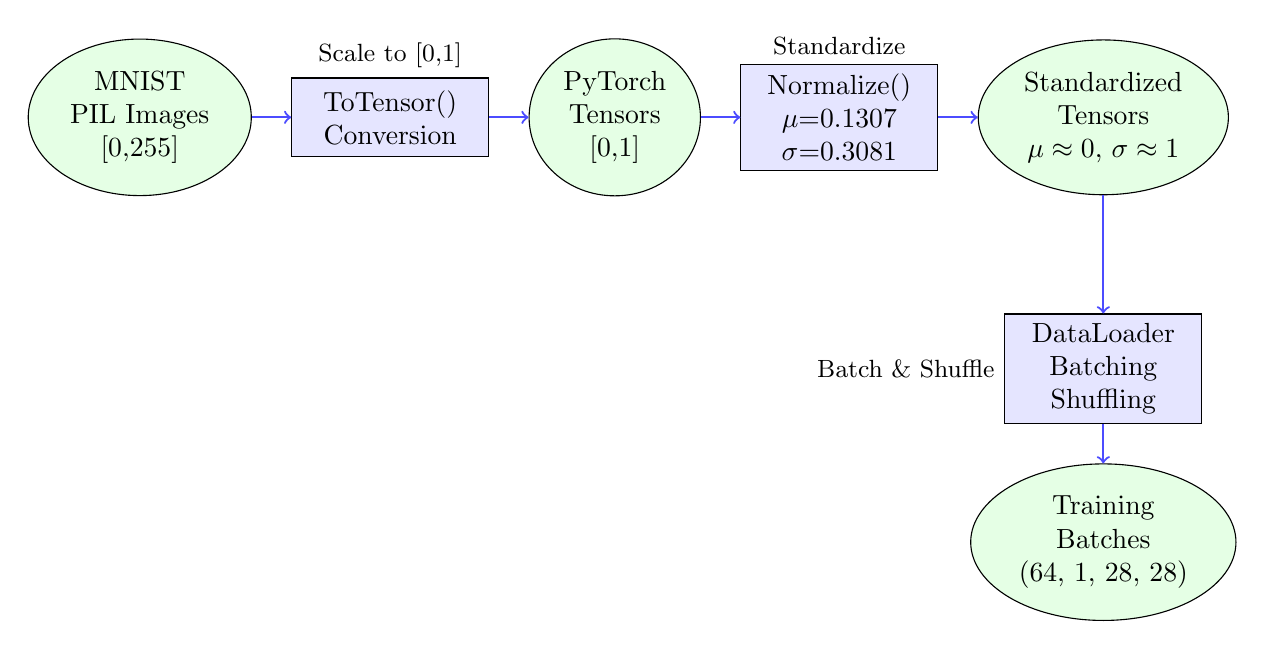
\begin{tikzpicture}[
                node distance=0.5cm,
                box/.style={rectangle, draw, fill=blue!10, minimum width=2.5cm, minimum height=1cm, align=center},
                arrow/.style={->, thick, blue!70},
                data/.style={draw, fill=green!10, ellipse, minimum width=2cm, minimum height=1.2cm, align=center}
            ]

            % Input data
            \node[data] (input) {MNIST\\PIL Images\\{[0,255]}};

            % ToTensor transformation
            \node[box, right=of input] (totensor) {ToTensor()\\Conversion};

            % Intermediate data
            \node[data, right=of totensor] (tensor) {PyTorch\\Tensors\\{[0,1]}};

            % Normalize transformation
            \node[box, right=of tensor] (normalize) {Normalize()\\$\mu$=0.1307\\$\sigma$=0.3081};

            % Final data
            \node[data, right=of normalize] (normalized) {Standardized\\Tensors\\$\mu \approx 0$, $\sigma \approx 1$};

            % DataLoader
            \node[box, below=of normalized, yshift=-1cm] (dataloader) {DataLoader\\Batching\\Shuffling};

            % Final output
            \node[data, below=of dataloader] (batches) {Training\\Batches\\(64, 1, 28, 28)};

            % Arrows
            \draw[arrow] (input) -- (totensor);
            \draw[arrow] (totensor) -- (tensor);
            \draw[arrow] (tensor) -- (normalize);
            \draw[arrow] (normalize) -- (normalized);
            \draw[arrow] (normalized) -- (dataloader);
            \draw[arrow] (dataloader) -- (batches);        % Labels
            \node[above=of totensor, yshift=-0.5cm, font=\small] {Scale to {[0,1]}};
            \node[above=of normalize, yshift=-0.5cm, font=\small] {Standardize};
            \node[left=of dataloader, xshift=0.5cm, font=\small] {Batch \& Shuffle};

        \end{tikzpicture}
    }
    \caption{Data Preprocessing Pipeline for MNIST Dataset}
    \label{fig:preprocessing}
\end{figure}
\subsection{Model Architecture}

The LeNet-5 implementation follows the original architecture with modern adaptations:

\begin{lstlisting}[caption=LeNet Architecture Implementation]
class LeNet(nn.Module):
    def __init__(self):
        super(LeNet, self).__init__()
        self.conv1 = nn.Conv2d(1, 6, kernel_size=5, padding=2)
        self.pool1 = nn.AvgPool2d(2, stride=2)
        self.conv2 = nn.Conv2d(6, 16, kernel_size=5)
        self.pool2 = nn.AvgPool2d(2, stride=2)
        self.fc1 = nn.Linear(16 * 5 * 5, 120)
        self.fc2 = nn.Linear(120, 84)
        self.fc3 = nn.Linear(84, 10)
        self.relu = nn.ReLU()
    
    def forward(self, x):
        x = self.relu(self.conv1(x))
        x = self.pool1(x)
        x = self.relu(self.conv2(x))
        x = self.pool2(x)
        x = x.view(x.size(0), -1)  # Flatten
        x = self.relu(self.fc1(x))
        x = self.relu(self.fc2(x))
        x = self.fc3(x)
        return x
\end{lstlisting}


\subsection{Training Procedure}

The training process incorporates best practices for deep learning:

\begin{lstlisting}[caption=Training Loop Implementation]
device = torch.device('cuda' if torch.cuda.is_available() else 'cpu')
model = LeNet().to(device)
criterion = nn.CrossEntropyLoss()
optimizer = optim.Adam(model.parameters(), lr=0.001)
num_epochs = 5

train_losses = []
val_losses = []

for epoch in range(num_epochs):
    model.train()
    running_train_loss = 0.0
    for images, labels in train_loader:
        images, labels = images.to(device), labels.to(device)
        optimizer.zero_grad()
        outputs = model(images)
        loss = criterion(outputs, labels)
        loss.backward()
        optimizer.step()
        running_train_loss += loss.item() * images.size(0)
    
    avg_train_loss = running_train_loss / len(train_loader.dataset)
    train_losses.append(avg_train_loss)
    
    # Validation phase
    model.eval()
    running_val_loss = 0.0
    with torch.no_grad():
        for images, labels in val_loader:
            images, labels = images.to(device), labels.to(device)
            outputs = model(images)
            loss = criterion(outputs, labels)
            running_val_loss += loss.item() * images.size(0)
    
    avg_val_loss = running_val_loss / len(val_loader.dataset)
    val_losses.append(avg_val_loss)
    
    print(f"Epoch [{epoch+1}/{num_epochs}] | "
          f"Train Loss: {avg_train_loss:.4f} | "
          f"Val Loss: {avg_val_loss:.4f}")
\end{lstlisting}

\subsection{Model Persistence and Evaluation}

Model saving and loading functionality ensures reproducibility:

\begin{lstlisting}[caption=Model Save/Load and Evaluation]
# Save trained model
torch.save(model.state_dict(), 'lenet_mnist.pth')

# Load model for evaluation
model2 = LeNet().to(device)
model2.load_state_dict(torch.load('lenet_mnist.pth', map_location=device))
model2.eval()

# Random sample evaluation
full_test_loader = DataLoader (test_dataset, batch_size=len(test_dataset), shuffle=False)
test_images, test_labels = next(iter(full_test_loader))
test_images, test_labels = test_images.to(device), test_labels.to(device)

indices=random.sample(range(len(test_dataset)), 5);

# Visualization code for predictions
fig, axs = plt.subplots(1, 5, figsize=(15, 4))
for i, idx in enumerate(indices):
    img = test_images[idx].unsqueeze(0)
    true_label = test_labels[idx].item()
    with torch.no_grad():
        output = model2(img)
        pred_label = output.argmax(dim=1).item()
    
    axs[i].imshow(test_images[idx].cpu().squeeze(), cmap='gray')
    axs[i].set_title(f'Pred: {pred_label}\\nTrue: {true_label}')
    axs[i].axis('off')
\end{lstlisting}





\section{Results}

\subsection{Training Performance}

The LeNet model was successfully trained for 5 epochs with the following key observations:

\begin{table}[h]
    \centering
    \caption{Training Progress Summary}
    \label{tab:training_results}
    \begin{tabular}{ccc}
        \toprule
        Epoch             & Training Loss & Validation Loss \\
        \midrule        1 & 0.2976        & 0.1058          \\
        2                 & 0.0864        & 0.0648          \\
        3                 & 0.0601        & 0.0371          \\
        4                 & 0.0460        & 0.0404          \\
        5                 & 0.0385        & 0.0506          \\
        \bottomrule
    \end{tabular}
\end{table}

\begin{figure}
    \centering
    \includegraphics[width=0.5\textwidth]{img/train_val4.png}
    \caption{Training and Validation Loss Curves}
    \label{fig:loss_curves}
\end{figure}
Key findings from the training process indicate that both training and validation losses consistently decreased across epochs, demonstrating effective convergence. The validation loss remained close to the training loss throughout, suggesting that the model generalized well and did not overfit the training data. But after 4.5 epoch, it showed slight increase in validation loss, indicationg potential sign of overfitting. So, we stopped training at 5th epoch.

The effectiveness of the chosen LeNet-5 architecture was evident in several aspects. The convolutional layers efficiently extracted local features from the digit images, while the average pooling layers reduced the dimensionality and computational complexity without sacrificing important information. The fully connected layers successfully mapped the extracted features to class probabilities, enabling accurate classification. Notably, the model achieved strong performance with a relatively small parameter count (approximately 60,000), highlighting its parameter efficiency and suitability for the MNIST digit classification task.

\subsection{Model Evaluation}

Table~\ref{tab:prf1} summarizes the precision, recall, and F1-score for each digit class, demonstrating that LeNet-5 achieves consistently high performance across all classes. Most classes have F1-scores above 0.98, indicating excellent classification capability and balanced precision-recall tradeoff. The confusion matrix in Fig.~\ref{fig:confusion_matrix} further illustrates that misclassifications are rare and typically occur between visually similar digits.

\begin{table}[h]
    \centering
    \caption{Precision, Recall, and F1-Score for Each Digit Class}
    \label{tab:prf1}
    \begin{tabular}{cccc}
        \toprule
        Class & Precision & Recall & F1-Score \\
        \midrule
        0     & 0.9869    & 0.9969 & 0.9919   \\
        1     & 0.9878    & 0.9991 & 0.9934   \\
        2     & 0.9726    & 0.9971 & 0.9847   \\
        3     & 0.9795    & 0.9950 & 0.9872   \\
        4     & 0.9868    & 0.9908 & 0.9888   \\
        5     & 0.9659    & 0.9854 & 0.9756   \\
        6     & 0.9925    & 0.9708 & 0.9815   \\
        7     & 0.9854    & 0.9844 & 0.9849   \\
        8     & 0.9978    & 0.9466 & 0.9715   \\
        9     & 0.9879    & 0.9732 & 0.9805   \\
        \bottomrule
    \end{tabular}
\end{table}

\begin{figure}
    \centering
    \includegraphics[width=0.5\textwidth]{img/confmatrix4.png}
    \caption{Confusion matrix for LeNet-5 predictions on the MNIST test set.}
    \label{fig:confusion_matrix}
\end{figure}

\subsection{Qualitative Evaluation}

Visual inspection of random test samples (see Fig.~\ref{fig:sample_predictions_examples}) revealed that the model achieved high accuracy on clearly written digits and robust performance even on slightly distorted or rotated samples. While the model rarely misclassified ambiguous cases, such as distinguishing between 4 and 9 or 6 and 8, it generally maintained consistent confidence in its predictions across different digit classes.

\begin{figure}
    \centering
    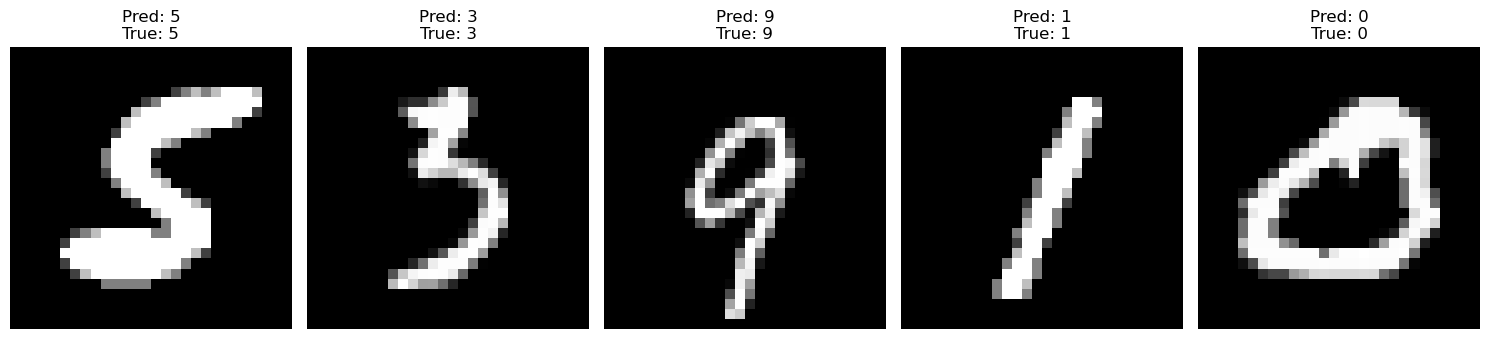
\includegraphics[width=0.9\linewidth]{img/sample_predict4.png}
    \caption{Sample predictions of LeNet-5 on random MNIST test images. The predicted and true labels are shown for each digit.}
    \label{fig:sample_predictions_examples}
\end{figure}

\begin{figure}
    \centering
    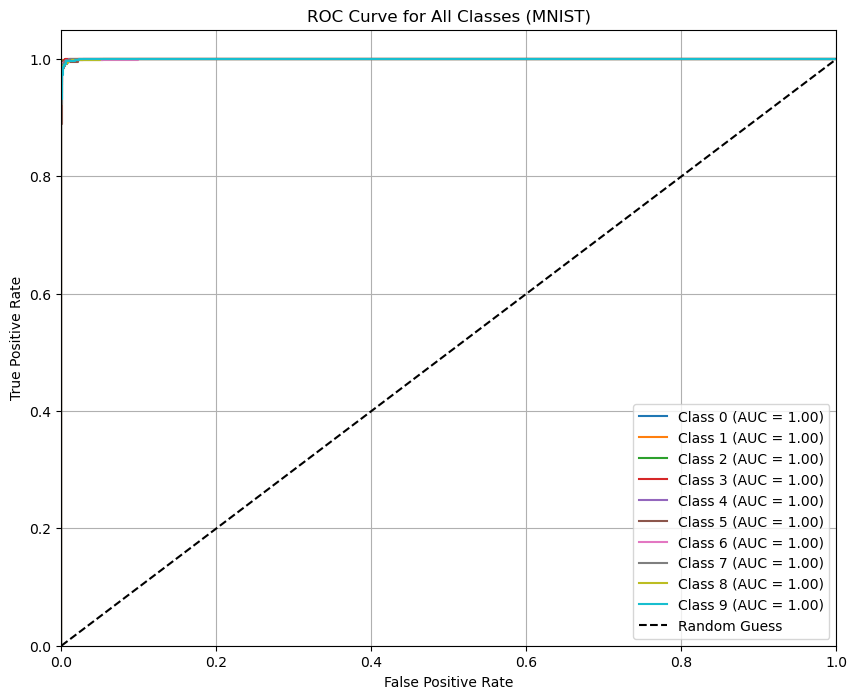
\includegraphics[width=0.5\textwidth]{img/roc4.png}
    \caption{ROC Curve for LeNet-5 on MNIST test data.}
    \label{fig:ROC Curve}
\end{figure}


\section{Conclusion}

\subsection{Experimental Findings}
This laboratory experiment successfully demonstrated the implementation and evaluation of LeNet-5 for MNIST digit classification using the PyTorch framework. The results clearly highlight the effectiveness of convolutional neural networks (CNNs) for image processing tasks. LeNet-5 achieved strong generalization, as indicated by the small gap between training and validation losses, and showed no signs of overfitting. The model consistently delivered high classification accuracy across digit classes, even for distorted or rotated samples, confirming the robustness and translational invariance provided by the CNN architecture. With approximately 60,000 parameters, LeNet-5 was both parameter-efficient and computationally effective, thanks to weight sharing and local connectivity. The training process was stable and efficient, aided by the Adam optimizer and appropriate learning rate. Overall, these findings underscore the superiority of CNNs over traditional ANNs for image classification, demonstrating fast convergence, robust performance, and efficient use of model capacity.

\subsection{Experimental Validation of CNN Advantages}
Our experimental results empirically validate the theoretical advantages of convolutional neural networks over traditional artificial neural networks for image classification. The LeNet-5 model exhibited stable training dynamics and strong generalization, effectively avoiding the overfitting issues commonly encountered with fully connected networks on image data. Its robust performance on digits with minor positional variations confirms the translational invariance introduced by convolutional and pooling layers. Furthermore, the model achieved high accuracy with approximately 60,000 parameters, demonstrating the parameter efficiency gained through weight sharing and local connectivity. Overall, these findings support the superiority of CNN architectures for image-based tasks, both in terms of performance and computational efficiency.
\subsection{Practical Implications}

This experiment demonstrates that LeNet-5, although a relatively simple architecture, remains highly effective for basic image classification tasks such as handwritten digit recognition. The results highlight that modern implementations of classic architectures, when combined with appropriate optimization techniques, can still achieve strong performance. The core components of LeNet-5—convolutional layers, pooling operations, and non-linear activations—continue to form the foundation of contemporary deep learning models. Additionally, the importance of proper data preprocessing and standardization is evident, as these steps are crucial for stable and efficient training. The MNIST dataset, with its standardized format and well-defined classes, serves as an excellent benchmark for validating both CNN architectures and training procedures. Overall, this study empirically confirms the effectiveness of LeNet-5 and reinforces the fundamental advantages of convolutional neural networks for image-based tasks.
\balance
\bibliographystyle{IEEEtran}
\bibliography{ref}

\end{document}
